% This is the template Jun uses for project seeds
% jun.allard@uci.edu allardlab.com
\documentclass[onecolumn,11pt]{article}

% --------- required packages ---------
\usepackage{enumerate}
\usepackage{enumitem}
\usepackage{graphicx}
\usepackage[colorlinks,allcolors=black]{hyperref}
\usepackage[font=small]{caption}

% Units, define microMolar, picoNewton, micron, etc.
\usepackage{siunitx}
\sisetup{per-mode=reciprocal} % Change here to get slash or ^{-1}
\DeclareSIUnit{\million}{\text{million}}
\DeclareSIUnit{\Units}{\text{Units}}
\DeclareSIUnit{\cells}{\text{cells}}
\DeclareSIUnit{\well}{\text{well}}
\DeclareSIUnit\Molar{\mole\per\cubic\deci\metre}
\DeclareSIUnit\Molar{\textsc{m}}
\newcommand{\uM}{\si{\micro\Molar}}
\newcommand{\um}{\si{\micro\metre}}
\newcommand{\pN}{\si{\pico\newton}}
\newcommand{\s}{\si{\second}}
\newcommand{\nm}{\si{\nano\metre}}

\usepackage{times}  
\usepackage{titlesec}      

\usepackage{titling}
\usepackage{authblk} % must come after titling package loading

% --------- standard packages ---------
%\usepackage{amsfonts}
\usepackage{amsmath}      
\usepackage{amssymb} 
%\usepackage{array}  
%\usepackage{bm}
%\usepackage{color}
%\usepackage{chemarr}
%\usepackage{float} 
\usepackage[utf8]{inputenc}
\usepackage{lipsum}
%\usepackage{mathtools}
%\usepackage{multicol}
%\usepackage{multirow}
%\usepackage{pdfsync}
%\usepackage{tocloft}
\usepackage{verbatim} % This also provides the \comment{} environment
\renewcommand{\comment}[1]{{\textcolor{blue}{{#1}}}}

%\usepackage{wrapfig}


% --------- packages, less often used ---------
%\usepackage[export]{adjustbox}
%\usepackage{amsopn}
%\usepackage{cancel} % adds strikethrough
%\usepackage{CJK} % Chinese Japanese Korean
%\usepackage{dcolumn} % align columns in a table
%\usepackage{dsfont}
%\usepackage{epsfig}
%\usepackage{epstopdf}
%\usepackage{esint} % integrals
%\usepackage{framed}
%\usepackage{physics} %for \vqty, \dd, \dv
%\usepackage{rotating}
%\usepackage{setspace} % set space between lines
\usepackage{subcaption}

%\usepackage{tcolorbox}
%\usepackage[normalem]{ulem} % for underlining
% --------- for typesetting code blocks --------
%\usepackage{algorithmic} % for code including Matlab
%\usepackage{listings} % for code including Matlab
%\usepackage[numbered,framed,basicstyle]{matlab-prettifier}

%%%%%%%%%%%%%%%%%%%%%%%%%%%%%%%%%%%%%%%%%%%%%%%%%%%%%%%%%%%%
% page layout
\usepackage[margin=1in]{geometry}

% paragraph layout
\setlength{\parindent}{0pt} % paragraph indent - looks best zero
\setlength{\parskip}{0.8em plus 0.1em minus 0.1em} % paragraph spacing
\setlist[itemize]{itemsep=0.0em,topsep=0em}
\setlist[enumerate]{itemsep=0.0em,topsep=0em}
\titlespacing{\paragraph}{0em}{-0.8em}{1em} % for the /paragraph command

\clubpenalty10000
\widowpenalty10000

% \def\alphaoff{\alpha_{\mbox{\scriptsize off}}}
% \def\alphaon{\alpha_{\mbox{\scriptsize on}}}
% \def\cos2{\mbox{cos$^2$}}
% \def\sin2{\mbox{sin$^2$}}
% \def\tan2{\mbox{tan$^2$}}
% \def\aka{\emph{a.k.a. }}
% \def\boff{^b_{\mbox{\scriptsize off}}}
% \def\bon{^b_{\mbox{\scriptsize on}}}
% \def\bsub{\emph{B. subtilis}}
% \def\caul{\emph{C. crescentus}}
% \def\cosh{\mbox{cosh}\,}
% \def\cos{\mbox{cos}\,}
\def\deg{^\circ}
% \def\denovo{\emph{de novo}}
% \def\ds{\partial_s}
% \def\dt{\partial_t}
% \def\ecoli{\emph{E. coli}}
% \def\eg{\emph{e.g. }}
% \def\fcat{f_{cat}}
% \def\fgp{f_{gp}}
% \def\fgs{f_{gs}}
% \def\fpg{f_{pg}}
% \def\fps{f_{ps}}
% \def\fres{f_{res}}
% \def\fsg{f_{sg}}
% \def\fsp{f_{sp}}
% \def\fstall{f_{\mbox{\scriptsize stall}}}
% \def\ie{\emph{i.e. }}
% \def\invitro{\emph{in vitro}}
% \def\invitro{{in vitro}}
% \def\invivo{\emph{in vivo}}
% \def\invivo{{in vivo}}
% \def\kback{k_{back}}
% \def\kboff{k^b_{\mbox{\scriptsize off}}}
% \def\kbon{k^b_{\mbox{\scriptsize on}}}
% \def\khyd{k_{\mbox{\scriptsize hyd}}}
% \def\khyd{k_{hyd}}
% \def\knuc{k_{nuc}}
% \def\koff{k_{\mbox{\scriptsize off}}}
% \def\kon{k_{\mbox{\scriptsize on}}}
% \def\kpoff{k^p_{\mbox{\scriptsize off}}}
% \def\kpon{k^p_{\mbox{\scriptsize on}}}
% \def\min{\,\mbox{min}}
% \def\muM{\,\mu\mbox{M}}
% \def\mum{\,\mu\mbox{m}}
% \def\nm{\,\mbox{nm}}
% \def\pN{\,\mbox{pN}}
% \def\pclaspbg{p_{\mbox{\scriptsize CLASP-bg}}}
% \def\pclasp{p_{\mbox{\scriptsize CLASP}}}
% \def\pcross0{p_{\mbox{\scriptsize cross}}^0}
% \def\pcrossAA{p_{\mbox{\scriptsize cross}AA}}
% \def\pcrossAP{p_{\mbox{\scriptsize cross}AP}}
% \def\poff{^p_{\mbox{\scriptsize off}}}
% \def\poff{^p_{\mbox{\scriptsize off}}}
% \def\pon{^p_{\mbox{\scriptsize on}}}
% \def\pside{p_{\mbox{\scriptsize side}}}
% \def\rhod{\emph{R. sphaeroides}}
% \def\sech{\mbox{sech}\,}
% \def\sinh{\mbox{sinh}\,}
% \def\sin{\mbox{sin}\,}
% \def\s{\,\mbox{s}}
% \def\tan{\mbox{tan}\,}
% \def\therm{\emph{Thermotoga}}
% \def\vms{v^m_s}
% \def\vpg{v^p_g}
% \def\vps{v^p_s}
% \def\Ara{\emph{Arabidopsis}}
% \def\ara{\emph{Arabidopsis}}
% \def\vfree{v_{\mbox{\scriptsize free}}}
% \def\vpoly{v_{\mbox{\scriptsize poly}}}
% \def\Fstall{F_{\mbox{\scriptsize stall}}}
%Frequely used notations
\newcommand{\KD}{K\textsubscript{D}\xspace}
\newcommand{\koff}{$k$\textsubscript{off}\xspace}
\newcommand{\kon}{$k$\textsubscript{on}\xspace}
\newcommand{\ecf}{EC\textsubscript{50}\xspace}
\newcommand{\icf}{IC\textsubscript{50}\xspace}
% \newcommand{\approxt}{{$\sim$}}
% \newcommand{\Ag}{\text{Ag}}
% \newcommand{\Agsur}{\text{Ag}_{\text{sur}}}
% \newcommand{\Ab}{\text{Ab}}
% \newcommand{\D}[2]{\frac{d#1}{d#2}}
% \newcommand{\Cp}{C_{\text{p}}}
% \newcommand{\ts}{t_{\text{s}}}
% \newcommand{\konm}{k_{\text{on}}}
% \newcommand{\khatonm}{\hat{k}_{\text{on}}}
% \newcommand{\koffm}{k_{\text{off}}}
% \newcommand{\konbm}{k_{\text{on,b}}}
% \newcommand{\ind}{\mathbbm{1}}
% \newcommand{\E}{\mathbb{E}}
% \newcommand{\avg}[1]{\E[#1]}
% \newcommand{\nocc}{\mathcal{N}}
% \newcommand{\Nag}{N_{\text{Ag}}}
% \newcommand{\Rp}{R_{\text{p}}}
% \newcommand{\vtheta}{\boldsymbol{\theta}}
% \newcommand{\Na}{N_{\text{A}}}
% \newcommand{\Rs}{R_{\text{s}}}
% \newcommand{\ubar}[1]{\underaccent{\bar}{#1}}
% \newcommand{\Nsims}{N_{\text{sims}}}
% \newcommand{\reach}{\varepsilon}
% \newcommand{\reachsur}{\reach_{\text{sur}}}
% \newcommand{\reachphys}{\reach_{\text{phys}}}



% Bibliography setup
\usepackage[numbers,square,sort&compress]{natbib}
\bibliographystyle{unsrtnat}
%\bibliographystyle{biophysj}

\title{JeanJacket main result statement as the title}
\author[a]{Jun}
\affil[a]{University of California Irvine}


%%%%%%%%%%%%%%%%%%%%%%%%%%%%%%%%%%%%%%%%%%%%%%%%%%%%%%%
\date{} % leave blank for no date
\begin{document}

\maketitle
%%%%%%%%%%%%%%%%%%%%%%%%%%%%%%%%%%%%%%%%%%%%%%%%%%%%%%%

\begin{abstract}
Nothing here yet
\end{abstract}

%%%%%%%%%%%%%%%%%%%%%%%%%%%%%%%%%%%%%%%%%%%%%%%%%%%%%%%
% \textbf{Key words:} 

% \textbf{Pre-print server:} biorxiv

% %\textbf{Open access:} 

% \clearpage

% \renewcommand{\abstractname}{Abstract:}
% \begin{abstract}

% \end{abstract}

% \renewcommand{\abstractname}{Significance Statement:}
% \begin{abstract}
% \end{abstract}

%\renewcommand{\abstractname}{Graphical abstract:}
%\begin{abstract}
%\begin{figure}[!htb]\vspace{-0.8cm}
%	\begin{center}
%	\hspace*{-0.25in}
%	\includegraphics[width=12cm]{figures/figGraphicalAbstract.pdf}\vspace{-0.5cm}
%    \captionsetup{labelformat=empty} 	\end{center}
%\end{figure} \setcounter{figure}{0}   
%\end{abstract}

%\clearpage
%\linenumbers
%%%%%%%%%%%%%%%%%%%%%%%%%%%%%%%%%%%%%%%%%%%%%%%%%%%%%%%



\section{Project seed}

\subsection*{Summary}
\paragraph{Background/major question} \lipsum[2]
\paragraph{Specific question, puzzle or hypothesis}\lipsum[2]
\paragraph{Here we}\lipsum[2]
\paragraph{Methods, tools, expertise, skills}\lipsum[2]
\paragraph{Expected results}\lipsum[2]
\paragraph{Outcomes and implications}\lipsum[2]


%%%%%%%%%%%%%%%%%%%%%%%%%%%%%%%%
\begin{figure}[h!]
\centering
\includegraphics[width=4.5in]{figures/figJeanJacket.pdf}
\caption{\label{fig:JeanJacketSchematic}An awesome model of a puzzling phenomenon}
\end{figure}
%%%%%%%%%%%%%%%%%%%%%%%%%%%%%%%%

\subsection{Candidate titles}
 
\begin{itemize}
\item Predictive dynamic modeling connects timescales of day-to-day gene expression and decade-scale disease progression of Alzheimer's Disease using $\mathbb{C}^\star$ algebras
\item Ito lemma and Boltzmann statistics provide a cost-effective treatment for cardiovascular disease
\item Hybrid Metropolis-Gillespie algorithm reveals a novel design for enhanced CAR-T therapy by dynamnic recruitment of non-effector molecular crowders to the T cell membranes
\item Comparative study of noncanonical protrusions and what they optimize
\item Accelerated tendon healing by morphological alterations to tenocyte projections
\end{itemize}

\subsection*{Basic model} 

\lipsum[2-5]  

\subsection*{Reading}
Papers marked with $^{\bullet}$ are of notable interest.
\begin{itemize}
\item Primarily modeling: \citet{Slaughter.2013}, \citet{Zhang.2019}, \citet{Ohadi.2019}
\item Review articles on the system \cite{kajdlkjsadjkl}
\item Primarily experimental
\end{itemize}


\subsection*{First steps} 

Test dimensions. 
Dimensional analysis. Pull the other cell with \SI{10}{\pico\newton\per\second}. Deviatoric stress \SI{7e3}{\pascal}. Inside a math environment $R=\SI{120}{\micro\meter}$. 
Something in inverse microMolar $10\uM^{-1}$, and force in $10\pN$ and distance in either $10\um$ or $10\nm$


\subsection{Figure subreferencing}

\begin{figure}[!ht]
        \centering
        \begin{subcaptiongroup}
                \includegraphics[width=174mm]{figures/figJeanJacket.pdf}
                \phantomcaption\label{subfig:heatmap}
                \phantomcaption\label{subfig:lattice}
                \end{subcaptiongroup}
        \captionsetup{subrefformat=parens}
        \caption{\label{fig:majorfig}\textbf{Interpretation sentence.}
                \subref{subfig:heatmap} A good caption for the heatmap. 
                \subref{subfig:lattice} A good caption for the lattice. 
                }
\end{figure}

We should be able to reference Figure~\ref{subfig:heatmap} and Figure~\ref{subfig:lattice} separately.

% Bibliography
%\bibliography{jeanjacket}
\bibliography{literature_jun_tmp}

%%%%%%%%%%%%%%%%%%%%%%%%%%%%%%%%%%%%%%%%%%%%%%%%%%%%%%%%%%%%%%%%%%%%%%%%%%%%%

% Supplemental
\clearpage
\setcounter{table}{0}
        \renewcommand{\thetable}{S\arabic{table}}%
\setcounter{figure}{0}
        \renewcommand{\thefigure}{S\arabic{figure}}%
\renewcommand{\listfigurename}{List of Supporting Figures}
\renewcommand{\contentsname}{List of Supporting Text}

%\section{Supplemental material}

%%%%%%%%%%%%%%%%%%%%%%%%%%%%%%%%
%\begin{figure}[h!t]
%\centering
%\includegraphics[width=4.5in]{figJeanJacket.pdf}
%\caption{This is a supplemental figure}
%\label{fig:DetailedJeanJacketSchematic}
%\end{figure}
%%%%%%%%%%%%%%%%%%%%%%%%%%%%%%%%

\end{document}
